\documentclass[border=5pt]{standalone}

\usepackage{mathpazo}
\usepackage{pgfplots}
\pgfplotsset{compat=1.8}

 % define the binom function
\tikzset{declare function={
            binom(\k,\n,\p)=\n!/(\k!*(\n-\k)!)*\p^\k*(1-\p)^(\n-\k);
            }
        }

\begin{document}

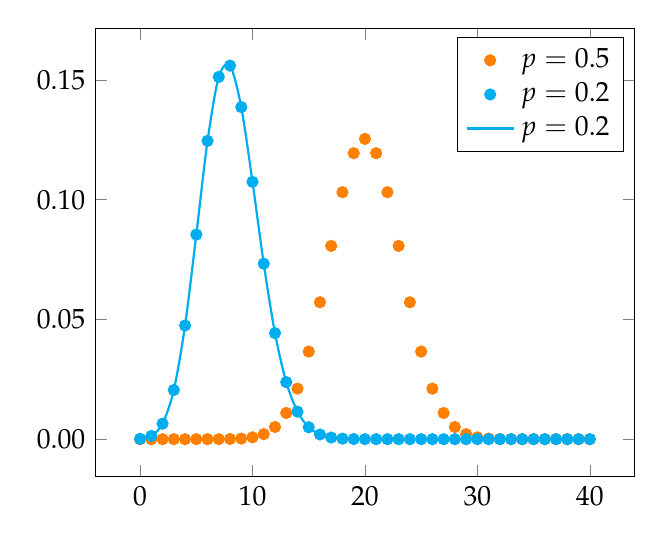
\begin{tikzpicture}
    \begin{axis}[samples at={0,...,40},
                 yticklabel style={
                   /pgf/number format/fixed,
                   /pgf/number format/fixed zerofill,
                   /pgf/number format/precision=2}
                ]
        \addplot [only marks,orange] {binom(x,40,0.5)};
        \addlegendentry{$p=0.5$}
        \addplot [only marks,cyan] {binom(x,40,0.2)};
        \addlegendentry{$p=0.2$}
        \addplot [smooth,thick,cyan] {binom(x,40,0.2)};
        \addlegendentry{$p=0.2$}
    \end{axis}
\end{tikzpicture}

\end{document}
